\documentclass[11pt,aspectratio=169]{beamer}
\usetheme{CambridgeUS}
\beamertemplatenavigationsymbolsempty
\usepackage{fontspec}
\setsansfont{Junicode}
\usepackage{amsmath,mathtools}
\usepackage{hyperref}
\usepackage{graphicx}
\usepackage{xpatch}
\usepackage[export]{adjustbox}
\usepackage{pgfplots}
\usepackage{tikz}
\usetikzlibrary{shapes,calc,matrix,decorations.markings,decorations.pathreplacing,positioning, intersections,backgrounds,through,hobby}
\usepackage{csquotes}
\usepackage[french]{babel}
\date[15/03/2024]{15 mars 2024}
\author[Matthias \textsc{Gille Levenson}]{{\Large Journée d'études \enquote{Cartographies ibériques du livre médiéval}}\\~\\ Matthias \textsc{Gille Levenson}\\   {\scriptsize École nationale des chartes -- CJM / École Normale Supérieure de Lyon - CIHAM}\\ {\tiny prénom [point] gille [tiret] levenson [at] ens-lyon [point] org}\vspace{-1cm}}
\title[Las marcas de lectura del mss. K.I.5]{Primeras pistas de estudio computacional de la recepción del \textit{Regimiento de los Prínçipes}.\\ \normalsize Las marcas de lectura del manuscrito K.I.5 (Biblioteca del Escorial).}
\titlegraphic{\vspace{-.5cm}\includegraphics[scale=0.18]{/home/mgl/Bureau/Travail/admin/logos/enc.png}\hspace{0.5cm}\includegraphics[scale=0.18]{/home/mgl/Bureau/Travail/admin/logos/ensl.png}\hspace{0.5cm}\includegraphics[scale=0.20]{/home/mgl/Bureau/Travail/admin/logos/logo-ciham.png}}


%\usepackage[labelformat=empty]{caption}
\setbeamertemplate{caption}{\insertcaption\par}

\usepackage[datamodel=thesis,citestyle=authoryear,isbn=true,
doi=true,backend=biber,language=french,url=true,sorting=nty,maxnames=15, maxcitenames=4]{biblatex}
\renewbibmacro{in:}{}
\renewcommand*{\bibfont}{\tiny} 
% http://mcclinews.free.fr/latex/introbeamer/elements_contenu.html
%\xapptobibmacro{cite}{\setunit{\nametitledelim}\printfield{year}}{}{}
\addbibresource{biblio.bib}

\begin{filecontents*}{thesis.dbx}
\ProvidesFile{thesis.dbx}[2014/06/14 supervisor for theses]
\RequireBiber[3]
\DeclareDatamodelFields[type=list,datatype=name]{supervisor}
\DeclareDatamodelEntryfields[thesis]{supervisor}
\end{filecontents*}


\begin{filecontents*}{french-thesis.lbx}
\ProvidesFile{french-thesis.lbx}[2014/06/14 english for thesis]
\InheritBibliographyExtras{french}
\NewBibliographyString{supervision,jointsupervision}
\DeclareBibliographyStrings{%
inherit           = {french},
supervision       = {{dirigée par}{dir\adddotspace }},
jointsupervision  = {{codirigée par}{codir\adddotspace }},
}
\end{filecontents*}

\DeclareLanguageMapping{french}{french-thesis}

\newbibmacro*{thesissupervisor}{%
  \ifnameundef{supervisor}{}{%
    \ifnumgreater{\value{supervisor}}{1}
      {\bibstring{jointsupervision}}
      {\bibstring{supervision}}
    \printnames{supervisor}}}

\xpatchbibdriver{thesis}
  {\printfield{type}}
  {\printfield{type}
   \newunit
   \usebibmacro{thesissupervisor}}
  {\typeout{yep}}
  {\typeout{no}}
  
% https://tex.stackexchange.com/a/184878 ajout direction thèse





\AtBeginSection[]
{\begin{frame}
 \frametitle{}  
 \tableofcontents[currentsection,
                  hideothersubsections,
                  subsubsectionstyle=show/show/show/hide
                   ]
 \end{frame} 
 }



\setbeamertemplate{sections/subsections in toc}[square]
\setbeamertemplate{bibliography item}[sqare]
\setbeamertemplate{itemize item}[square]
\setbeamertemplate{enumerate item}[square]
\setbeamertemplate{itemize subitem}[square]





\renewcommand*{\dotFFN}{}
\newcommand{\astfootnote}[1]{%
\let\oldthefootnote=\thefootnote%
\setcounter{footnote}{0}%
\renewcommand{\thefootnote}{\fnsymbol{footnote}}%
\footnote{#1}%
\let\thefootnote=\oldthefootnote%
}








\begin{document}
\maketitle





\begin{frame}
%\frametitle{Esquema} % Table of contents slide, comment this block out to remove it
\tableofcontents % Throughout your presentation, if you choose to use \section{} and \subsection{} commands, these will automatically be printed on this slide as an overview of your presentation
\end{frame}


\section*{Introducción}
\addtocontents{toc}{Introducción}
\begin{frame}{El \textit{Regimiento de los prínçipes}}
\begin{center}
\url{https://github.com/matgille/extraccion_marcas_lecturas}
\begin{itemize}
\item Traducción del \textit{De Regimine Principum} de Egidio Romano, escrito hacia 1276-80
\item Supuestamente traducido para la educación de Pedro I a encargo del entorno de Alfonso 11
\item Una tradición con más huellas de lectura que otras, como la francesa \parencite{perret_les_2011}.
\end{itemize}
\end{center}
\end{frame}


\begin{frame}{La versión B}
\begin{itemize}
\item Existen varias versiones del texto (A, B, C) \parencite{acero-durantez_VersionesTraduccionCastellana_2005}, y circulan esencialmente manuscritos con una glosa extensa
\item Aunque hay manuscritos sin glosa que corresponden, creo, a la versión original que debió existir sin las glosas \parencite{gillelevenson_RegimientoPrincipesSa_2023}
\end{itemize}
\end{frame}


\begin{frame}{El manuscrito K.I.5 del Escorial}

Imagen del manuscrito

\begin{itemize}
\item Pertenece a la versión B, con glosas y una traducción generalmente resumida
\item Un manuscrito muy peculiar en cuanto a sus características externas
\item Una gótica cursiva probablemente del siglo 15. 
\item marcas frecuentes, sin glosas marginales o interlineales
\end{itemize}
\end{frame}


\begin{frame}{El manuscrito K.I.5 del Escorial}
\begin{figure}
\begin{center}
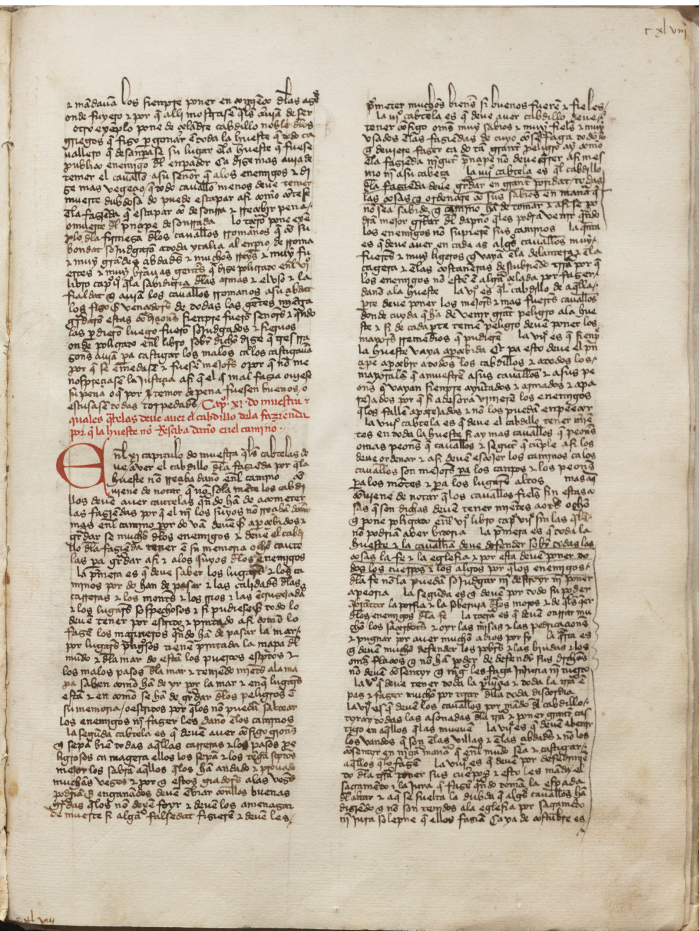
\includegraphics[height=.8\textheight]{/home/mgl/Bureau/Travail/Communications_et_articles/toulouse_mars/scripts/diapos/img/marca_2-2.png}
\caption{K.I.5, fol. 148r}
\end{center}
\end{figure}
\end{frame}



%\begin{frame}{Número de manos}
%Identifico dos manos principales:
%\begin{itemize}
%\item Mano 1
%\item Mano 2
%\end{itemize}
%\end{frame}


\begin{frame}{Tipos de marcas del K.I.5}
\begin{itemize}
\item Dos tipos de marcas verticales (a y b) 
\item Marcas horizontales: el texto viene subrayado con lápiz.
\end{itemize}
\end{frame}


\begin{frame}{Marcas verticales: tipo a}
\begin{center}
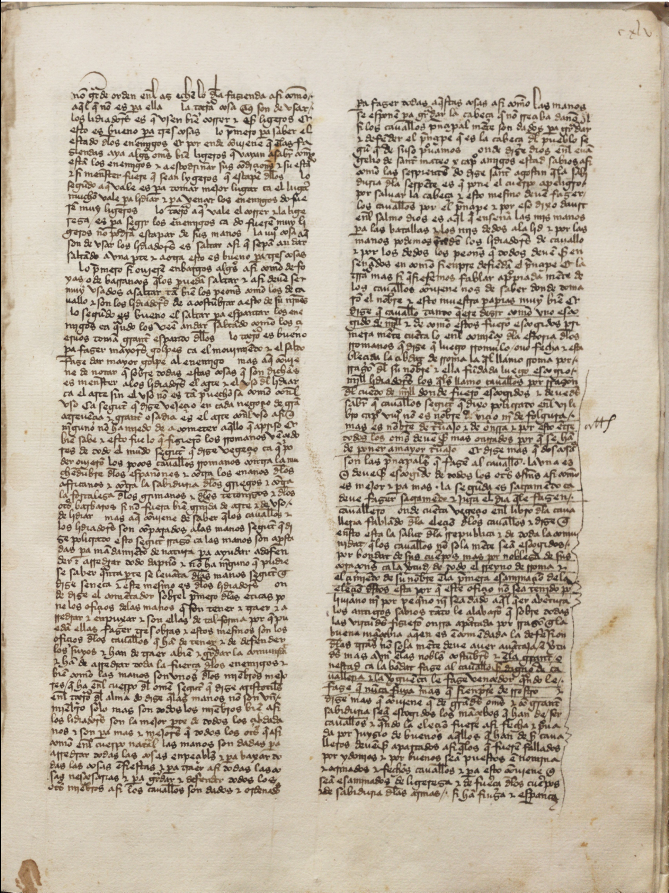
\includegraphics[height=.8\textheight]{/home/mgl/Bureau/Travail/Communications_et_articles/toulouse_mars/scripts/diapos/img/marca_2-1.png}
\end{center}
\end{frame}


\begin{frame}{Marcas verticales: tipo a}
\begin{center}
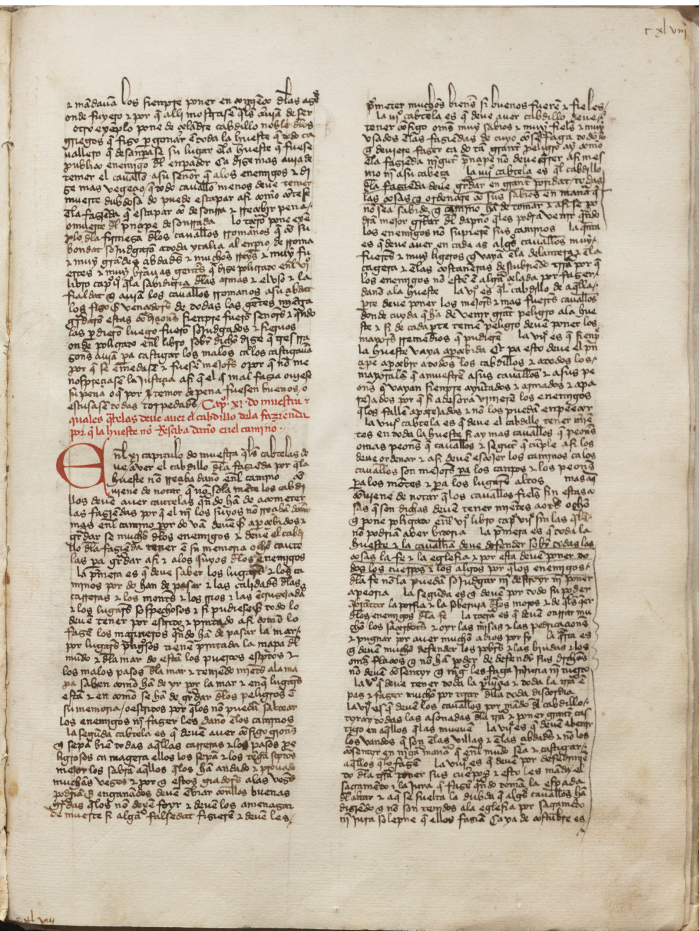
\includegraphics[height=.8\textheight]{/home/mgl/Bureau/Travail/Communications_et_articles/toulouse_mars/scripts/diapos/img/marca_2-2.png}
\end{center}
\end{frame}




\begin{frame}{Marcas verticales: tipo b}
\begin{center}
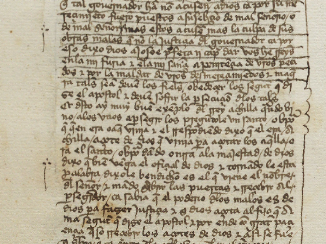
\includegraphics[height=.3\textheight]{/home/mgl/Bureau/Travail/Communications_et_articles/toulouse_mars/scripts/diapos/img/marca_3.png}
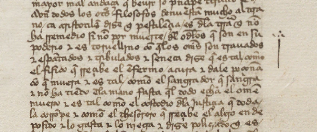
\includegraphics[height=.3\textheight]{/home/mgl/Bureau/Travail/Communications_et_articles/toulouse_mars/scripts/diapos/img/marca_3_2.png}
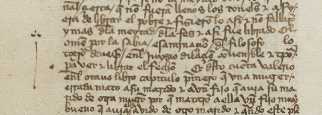
\includegraphics[height=.3\textheight]{/home/mgl/Bureau/Travail/Communications_et_articles/toulouse_mars/scripts/diapos/img/marca_3-3.png}
\end{center}
\end{frame}


\begin{frame}{Marcas horizontales}
\begin{center}
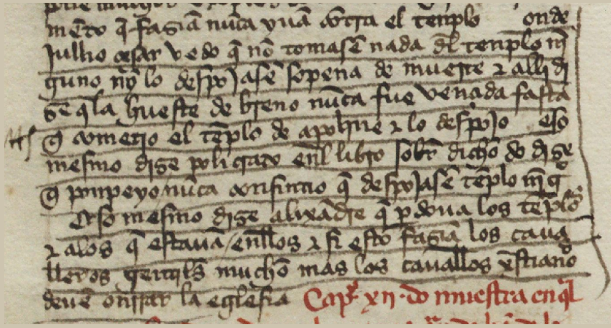
\includegraphics[height=.8\textheight]{/home/mgl/Bureau/Travail/Communications_et_articles/toulouse_mars/scripts/diapos/img/marca_horizontal_1.png}
\end{center}
\end{frame}

\begin{frame}{Marcas horizontales}
\begin{center}
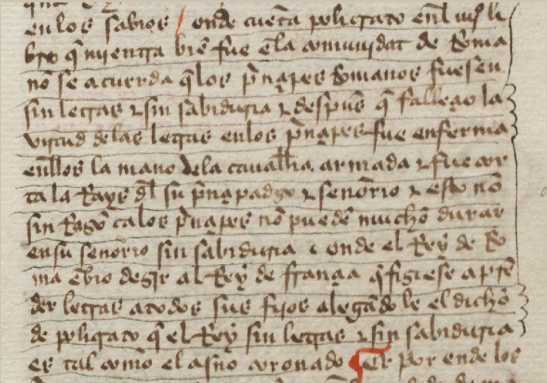
\includegraphics[height=.7\textheight]{/home/mgl/Bureau/Travail/Communications_et_articles/toulouse_mars/scripts/diapos/img/marca_horizontal_2.png}
\end{center}
\end{frame}

\begin{frame}{Marcas horizontales}
\begin{center}
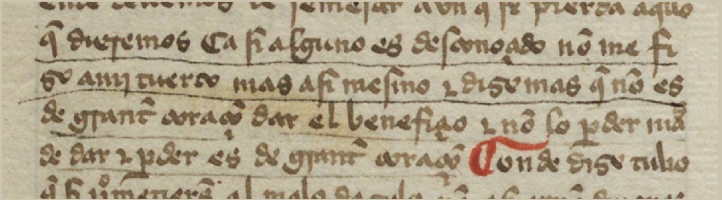
\includegraphics[height=.45\textheight]{/home/mgl/Bureau/Travail/Communications_et_articles/toulouse_mars/scripts/diapos/img/marca_horizontal_3.png}
\end{center}
\end{frame}



\begin{frame}{Tipos de marcas del K.I.5}
\begin{itemize}
\item No conocemos la identidad de la persona que anota, pero las marcas verticales de tipo a y los subrayados son de la misma mano; en general, ambas se completan. 
\item Las marcas verticales suelen cubrir mucho más texto. 
\item En cuanto a las marcas de tipo b, bastante frecuentes, es más difícil saberlo precisamente. 
\end{itemize}
\end{frame}

\begin{frame}{Orientaciones de estudio}
\begin{itemize}
\item ?`Qué nos dicen las marcas de lectura de los intereses de un lector del 15 o del 16?
\item ?`Podemos estudiar las marcas de manera exhaustiva, recuperando el texto anotado de manera semi-automática?
\item ?`Podemos identificar un programa de lectura preciso e intereses particulares?
\item ?`O es una lectura más general, centrándose en los elementos fundamentales de cada capítulo?
\end{itemize}
\end{frame}



%\section{Estado de la cuestión}
%\begin{frame}

%\end{frame}



\section{Métodos de extracción de los fragmentos anotados}

\begin{frame}{Tecnología: el aprendizaje supervisado}
\begin{itemize}
\item Las tres fases de la extracción hacen uso de una rama de la \enquote{inteligencia artificial}: el 
\textbf{aprendizaje supervisado}
\item Se trata de aprender a la máquina a resolver un problema dándole parejas de \textbf{\{datos + etiquetas\}}
\end{itemize}
\end{frame}

\subsection{Identificación de las marcas de lectura}

\begin{frame}{Herramienta y modelo de extracción de las marcas}
\begin{itemize}
\item Se utiliza un método de \textbf{detección de objetos} con la herramienta YOLOv8 \parencite{redmon_YouOnlyLook_2016}:
\begin{figure}
\begin{center}
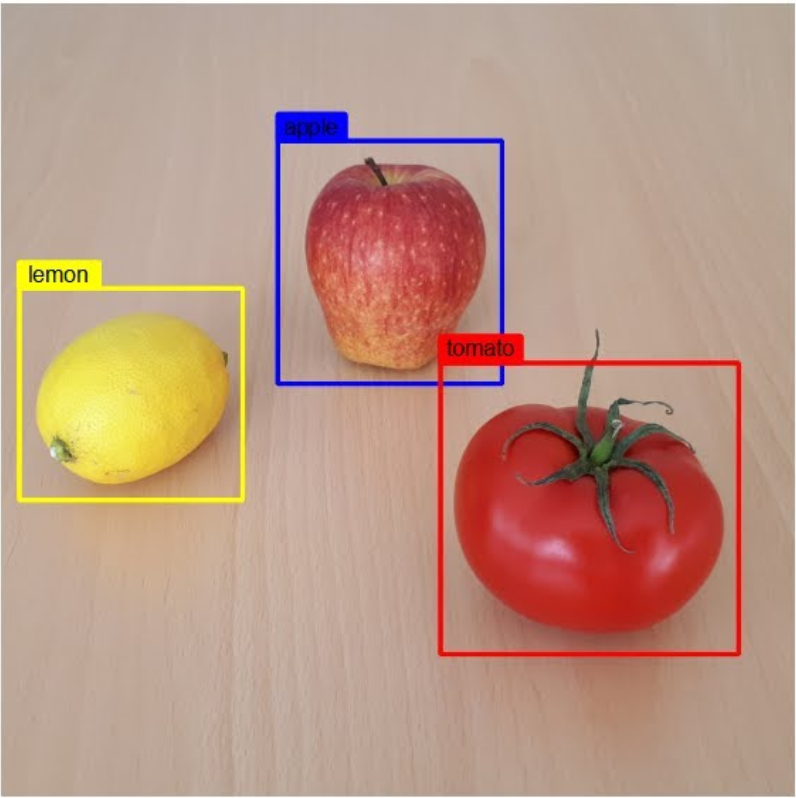
\includegraphics[height=.4\textheight]{img/yolo_detection.png}
% Cadea Youtube Computer Vision with Hüseyin Özdemir
\end{center}
\end{figure}
\item El modelo base se afina con 220 imágenes, o sea los 2/3 del corpus, lo que no es nada eficiente; sin embargo, el modelo se podrá reutilizar luego para ampliar el estudio.
\end{itemize}
\end{frame}


\begin{frame}{Un ejemplo de resultado}
\begin{center}
\includegraphics[height=.8\textheight]{/home/mgl/Bureau/Travail/Communications_et_articles/toulouse_mars/scripts/diapos/img/YOLO_identification.png}
\end{center}
\end{frame}


\begin{frame}{Resultados}
\begin{itemize}
\item Los resultados son bastante buenos, pero con los dos tercios del corpus transcrito a mano, y el último segmentado automáticamente
\item 153 marcas tras corrección. 
\item El modelo identifica correctamente todas las marcas pero es algunas identificaciones múltiples
\end{itemize}
\end{frame}


\subsection{Segmentación del fragmento anotado}

\begin{frame}{Herramienta y modelo de segmentación utilizado}
\begin{itemize}
\item El motor de segmentación kraken es utilizado como base. 
\item Se afina el modelo general con una 27 páginas segmentadas a mano
\end{itemize}
\end{frame}

\begin{frame}{Un ejemplo de resultado de segmentación}
\begin{center}
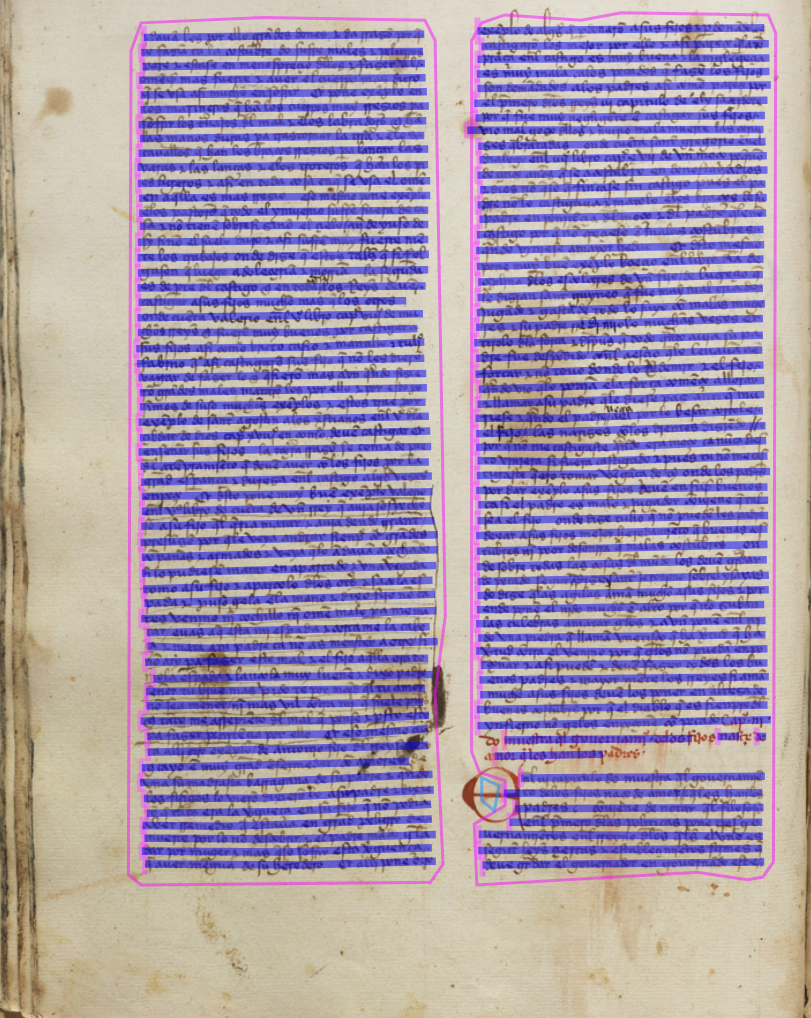
\includegraphics[height=.8\textheight]{/home/mgl/Bureau/Travail/Communications_et_articles/toulouse_mars/scripts/diapos/img/segmentation_results.png}
\end{center}
\end{frame}


\subsection{Transcripción del fragmento segmentado}

\begin{frame}{Herramienta y modelo de transcripción utilizado}
\begin{itemize}
\item Se utiliza el motor de transcripción Kraken \parencite{kiessling_KrakenUniversalText_2019} y el modelo CATMuS como base: 10 lenguas, siglos 7-14, corpus de entrenamiento de 160.000 líneas \parencite{clerice_CATMuSMedievalMultilingual_2024}.\\
\begin{center}

\includegraphics[scale=.3]{img/catmus.png}
\end{center}
\item El juego de datos de CATMuS tiene muy poca cursiva, y se tiene que adaptar el modelo a las escrituras del manuscrito con unas \textbf{1500 líneas}, en parte sin marcas, en parte con marcas
\item Dos problemas:
\begin{enumerate}
\item La gótica cursiva en sí
\item Las propias marcas que vienen dificultar la lectura
\end{enumerate} 
\end{itemize}
\end{frame}


\begin{frame}{Resultados}
\begin{itemize}
\item Los resultados son un poco decepcionantes para una lectura fina del texto, pero sirven para lectura distante
\item Esto se debe claramente a las marcas de lectura: el modelo es mucho mejor con el texto sin marcas, y los errores de segmentación y transcripción se combinan.
\end{itemize}
\end{frame}


\begin{frame}{Ejemplo de transcripción de buena calidad}
\begin{center}
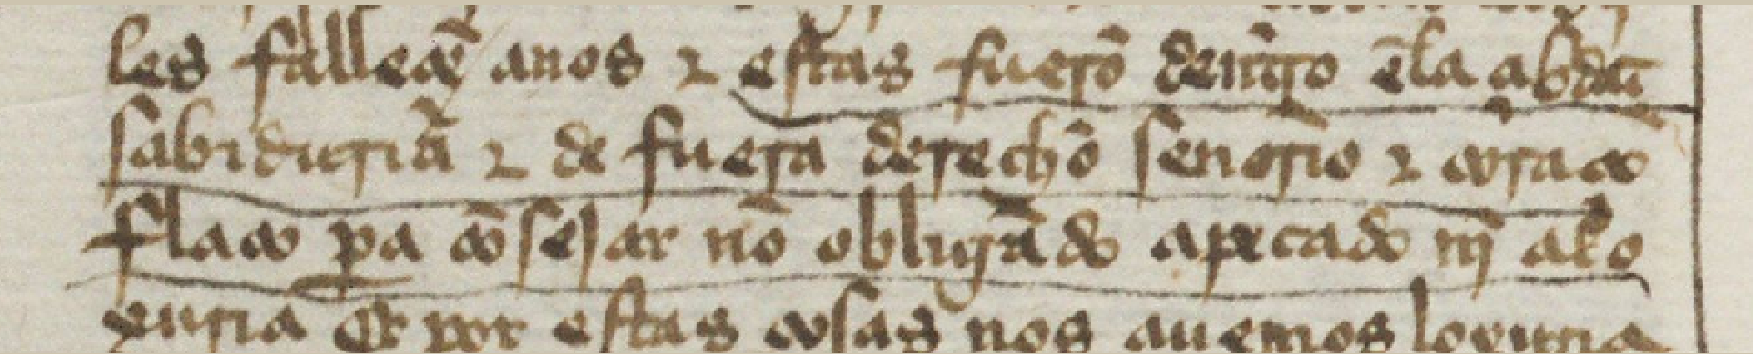
\includegraphics[width=.8\textwidth]{/home/mgl/Bureau/Travail/Communications_et_articles/toulouse_mars/scripts/diapos/img/ejemplo_transcripcion_buena.png}
\begin{quote}
les falleçẽ anos e estas fuerõ dentro ẽla çibdar
\\sabiduriã e de fuerã derechõ senorio e coraço
\\flaco ꝑa cõsejar nõ obligãdo aipecado nĩ alo
\\xũria et por estas cosas nos auemos loxuria
\end{quote}
Una vez normalizado: 
\begin{quote}
les fallecen a nos e estas fueron dentro enla cibdar sabidurian e de fueran derecho senorio e corazo flaco para consejar non obligando ai pecado nin aloxunria et por estas cosas nos auemos loxuria
\end{quote}
\end{center}
\end{frame}


\begin{frame}{Ejemplo de transcripción de mala calidad}
\begin{center}
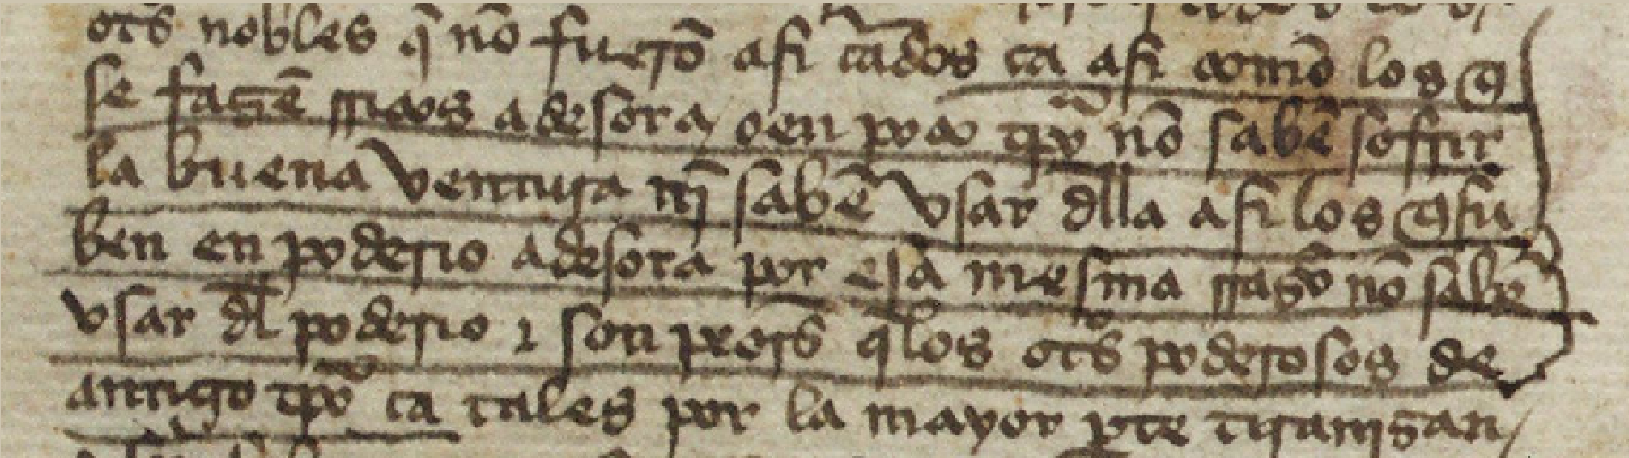
\includegraphics[width=.6\textwidth]{/home/mgl/Bureau/Travail/Communications_et_articles/toulouse_mars/scripts/diapos/img/ejemplo_mala_transcripcion.png}
\begin{quote}
otͦs nobles q̃ nõ fuerõ asi cãdos ca asi com̃o los q̃
\\efaçiẽ rriçes adesora oen poco tpx̃ nõ sabẽ sofrir
\\a buena ventura
\\bẽ
\\vsar dłla asi los al
\\den en poderio adesora por esa mesma rrapo nõ sabe
\\osar d̃ł poderio e son peorõ q̃los otͦs poderosos de
\\antigo tp̃o ca tales por la mayor ꝑte tiranizan/
\end{quote}
\end{center}
\end{frame}



\section{Resultados}


\begin{frame}{Lectura distante, lectura atenta}
\begin{center}
\begin{itemize}
\item Moretti
https://voyant-tools.org/?corpus=efc7db2029a3618d1658ce3e2d9b2069
https://voyant-tools.org/?corpus=651c3dcd301dffe6018d341cfd5a952a
\end{itemize}
\end{center}
\end{frame}



\subsection{Lectura distante: comparación de las frecuencias relativas de algunos términos}


\begin{frame}{Metodología}
\begin{center}
\begin{itemize}
\item Transcripción del texto de cada anotación
\item Normalización y desarrollo de abreviaturas
\item Lematización con Freeling
\item Recuperación de las frecuencias y comparación con las frecuencias del texto completo \textbf{lematizado} (base: incunable, edición de 1494 de Ungut y Polono)
\end{itemize}
\end{center}
\end{frame}


\begin{frame}{Estadísticas básicas del corpus}
\begin{center}
\begin{itemize}
\item 360.000 palabras en el texto completo (base incunable)
\item 10.000 palabras recuperadas en las marcas
\end{itemize}
\end{center}
\end{frame}


\begin{frame}{Comparación de frecuencias}
\begin{center}
\begin{itemize}
\item La idea es conseguir las \textbf{frecuencias relativas} de cada lema (= número de ocurrencias divido por el tamaño del corpus), y comparar estas frecuencias con las frecuencias del texto completo, para identificar alguna especificidad léxica
\end{itemize}
\end{center}
\end{frame}


\begin{frame}{Métricas utilizadas}
\begin{center}
\begin{itemize}
\item Frecuencia absoluta (lemas): número de ocurrencia de un lema en el corpus
\item Frecuencia relativa: $\frac{Frequencia\ absoluta\ (lemas)}{tama\tilde{n}o\ del\ corpus}$
\item Frecuencia comparada: $\frac{Frequencia\ relativa\ (lemas)\ texto\ marcas}{Frequencia\ relativa\ (lemas)\ texto\ completo}$
\item Si la frequencia comparada supera 1, el lema aparece -- en relativo -- más en las marcas que en el texto completo
\end{itemize}
\end{center}
\end{frame}

\begin{frame}{Términos políticos}
\begin{center}

\begin{itemize}
\item Lo que interesa el lector es el actor político más que nada
\begin{table}[!ht]
    \centering
    \begin{tabular}{|l|l|l|l|l|}
    \hline
        \textbf{Lemma} & \textbf{Frec. abs. (fragm)} & \textbf{Frec. rel (fragm)} & \textbf{Frec. abs. (incunable)} & \textbf{Razón} \\ \hline
        príncipe & 32 & 0,0033 & 0,00128 & 2,58224 \\ \hline
        principado & 10 & 0,00103 & 0,00024 & 4,27991 \\ \hline
        rey & 60 & 0,0062 & 0,0043 & 1,44184 \\ \hline
        caballero & 21 & 0,00217 & 0,00117 & 1,85388 \\ \hline
        noble & 18 & 0,00186 & 0,00071 & 2,61203 \\ \hline
    \end{tabular}
\end{table}
\end{itemize}
\end{center}
\end{frame}


\begin{frame}{Nobles y nobleza}
\begin{center}
\begin{itemize}
\item La nobleza sin duda interesa particularmente el lector
\begin{table}[!ht]
    \centering
    \begin{tabular}{|l|l|l|l|l|}
    \hline
        \textbf{Lemma} & \textbf{Frec. abs. (fragm)} & \textbf{Frec. rel (fragm)} & \textbf{Frec. abs. (incunable)} & \textbf{Razón} \\ \hline
        hidalgo & 3 & 0,00031 & 0,00008 & 3,75681 \\ \hline
        caballería & 13 & 0,00134 & 0,00043 & 3,13962 \\ \hline
        caballero & 21 & 0,00217 & 0,00117 & 1,85388 \\ \hline
        jurar & 6 & 0,00062 & 0,00008 & 8,1147 \\ \hline
        espada & 6 & 0,00062 & 0,00014 & 4,31633 \\ \hline
        escudo & 1 & 0,0001 & 0,00004 & 2,41509 \\ \hline
        caballo & 1 & 0,0001 & 0,00015 & 0,69003 \\ \hline
    \end{tabular}
\end{table}
\end{itemize}
\end{center}
\end{frame}

\begin{frame}{El caballero}
\begin{center}
\begin{itemize}
\item El caballero no designa al que combate a caballo, sino el que ciñe la espada y es ordenado
\begin{table}[!ht]
    \centering
    \begin{tabular}{|l|l|l|l|l|}
    \hline
        \textbf{Lemma} & \textbf{Frec. abs. (fragm)} & \textbf{Frec. rel (fragm)} & \textbf{Frec. abs. (incunable)} & \textbf{Razón} \\ \hline
        hidalgo & 3 & 0,00031 & 0,00008 & 3,75681 \\ \hline
        caballería & 13 & 0,00134 & 0,00043 & 3,13962 \\ \hline
        caballero & 21 & 0,00217 & 0,00117 & 1,85388 \\ \hline
        jurar & 6 & 0,00062 & 0,00008 & 8,1147 \\ \hline
        espada & 6 & 0,00062 & 0,00014 & 4,31633 \\ \hline
        escudo & 1 & 0,0001 & 0,00004 & 2,41509 \\ \hline
    \end{tabular}
\end{table}
\end{itemize}
\end{center}
\end{frame}


\begin{frame}{Economía y gestión de la casa}
\begin{center}
\begin{itemize}
\item Poco interés por cuestiones de la segunda parte:
\begin{table}[!ht]
    \centering
    \begin{tabular}{|l|l|l|l|l|}
    \hline
        \textbf{Lemma} & \textbf{Frec. abs. (fragm)} & \textbf{Frec. rel (fragm)} & \textbf{Frec. abs. (incunable)} & \textbf{Razón} \\ \hline
        mujer & 9 & 0,00093 & 0,00193 & 0,48073 \\ \hline
        marido & 1 & 0,0001 & 0,00053 & 0,19658 \\ \hline
        siervo & 3 & 0,00031 & 0,00087 & 0,35716 \\ \hline
        hijo & 17 & 0,00176 & 0,00221 & 0,79501 \\ \hline
        padre & 7 & 0,00072 & 0,00126 & 0,57586 \\ \hline
        castigo & 1 & 0,0001 & 0,00028 & 0,36356 \\ \hline
        casa & 3 & 0,00031 & 0,00108 & 0,28654 \\ \hline
        dinero & 1 & 0,0001 & 0,00039 & 0,2621 \\ \hline
    \end{tabular}
\end{table}
\end{itemize}

\end{center}
\end{frame}



\begin{frame}{Términos morales}
\begin{center}

\begin{itemize}
\item Interés por nociones básicas de bien y de mal
\item Poco interés por las virtudes
\end{itemize}

\end{center}
\end{frame}


\subsection{Distribución de las marcas en el manuscrito}
\begin{frame}{Número de marcas por parte y capítulo}
\begin{table}[!ht]
    \centering
    \begin{tabular}{|l|l|l|l|l|}
    \hline
        \textbf{Parte} & \textbf{Capítulos} & \textbf{Marcas} & \textbf{Ratio} & \textbf{Tema} \\ \hline
        \textbf{I, 1} & 13 & 0 & 0 & La bienaventuranza del príncipe \\ \hline
        \textbf{I, 2} & 34 & 27 & 0,79412 & Las virtudes \\ \hline
        \textbf{I, 3} & 11 & 4 & 0,36364 & Las pasiones \\ \hline
        \textbf{I, 4} & 7 & 23 & 3,28571 & Las costumbres de los reyes \\ \hline
        \textbf{II, 1} & 24 & 9 & 0,375 & Las mugeres \\ \hline
        \textbf{II, 2} & 22 & 9 & 0,40909 & Los fijos \\ \hline
        \textbf{II, 3} & 20 & 18 & 0,9 & Los siervos \\ \hline
        \textbf{III, 1} & 20 & 8 & 0,4 & La opinión de los filósofos sobre la Ciudad \\ \hline
        \textbf{III, 2} & 36 & 32 & 0,88889 & El gobierno en tiempos de paz \\ \hline
        \textbf{III, 3} & 23 & 21 & 0,91304 & El gobierno en tiempos de guerra \\ \hline
        \textbf{Total} & \textbf{210} & \textbf{151} & \textbf{0,80749} & ~ \\ \hline
    \end{tabular}
\end{table}
\end{frame}




\subsection{Orientaciones de la lectura: algunos ejemplos}
\begin{frame}{Parte I, 4: \enquote{De las costumbres de los reyes}}
\begin{itemize}
\item 24 marcas
\item Un apego a la nobleza ante todo y a la defensa de la idea de superioridad de la nobleza (16 marcas)
\item 112.0; 112.1;116.0 (sobre la riqueza sin nobleza)
\item \begin{center}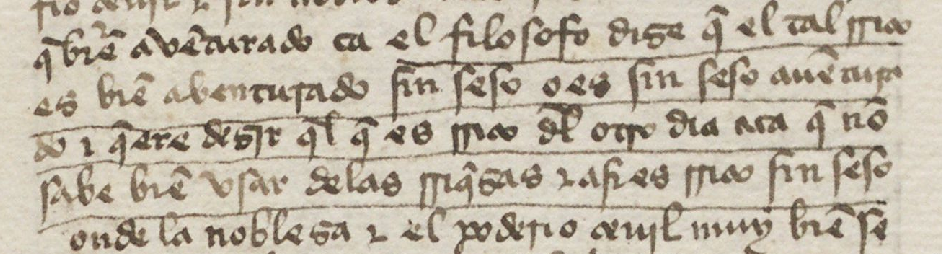
\includegraphics[width=.6\textwidth]{../results/kraken_transcription_results/pg_0116_0.png}\end{center}
\end{itemize}
\end{frame}

\begin{frame}{Parte II, 3: \enquote{El gobierno de los siervos}}
\begin{itemize}
\item 18 marcas
\end{itemize}
\end{frame}



\section*{Conclusiones}
\addtocontents{toc}{Conclusiones}

\begin{frame}{Un programa de lectura coherente}
\begin{center}
\begin{itemize}
\item Una lectura política clara y constante del texto
\item La nobleza 
\end{itemize}
\end{center}
\end{frame}


\begin{frame}{Por hacer}
\begin{center}
\begin{itemize}
\item Ampliar el estudio a los otros tipos de marcas y a otros manuscritos
\item Añadir una fase de corrección del texto
\end{itemize}
\end{center}
\end{frame}




\begin{frame}{Preguntas para el futuro}
\begin{center}
\begin{itemize}
\item Confirman estas observaciones las marcas verticales, probablemente producidas por la misma mano? 
\item Podemos precisar la localización de las marcas, en la glosa o en la traducción ?
\item Podemos ampliar el estudio a otros manuscritos para comparar los intereses de lectura?
\end{itemize}
\end{center}
\end{frame}


\begin{frame}{Gracias}
\begin{center}
Gracias por la atención !
\end{center}
\end{frame}



\begin{frame}[allowframebreaks]{Références}
\printbibliography
\end{frame}

\end{document}
